% -*- TeX-engine: xetex; TeX-PDF-mode: t -*-

\documentclass[a4paper, 14pt]{matmex-diploma-custom}

\usepackage[backend=biber]{biblatex}
\addbibresource{main.bib}

\begin{document}

\filltitle{ru}{
    chair              = {Кафедра Системного Программирования},
    title              = {Анализ эмоциональной окраски сообщений \\в микроблогах с помощью вероятностных моделей},
    type               = {diploma},
    position           = {студенки},
    group              = 545,
    author             = {Лебедева Екатерина Андреевна},
    supervisorPosition = {ст.преподаватель},
    supervisor = {Луцив Д.\,В.},
    reviewerPosition   = { },
    reviewer           = {Тузова Е.\,А.},
    chairHeadPosition  = {д.\,ф.-м.\,н., профессор},
    chairHead          = {Терехов А.\,Н.},
%   university         = {Санкт-Петербургский Государственный Университет},
%   faculty            = {Математико-механический факультет},
%   city               = {Санкт-Петербург},
   year               = {2014}
}

\filltitle{en}{
    chair              = {Software Engineering Chair},
    title              = {Sentiment analysis of microblog data via probabilistic models},
    author             = {Ekaterina Lebedeva},
    supervisorPosition = {senior lecturer},
    supervisor         = {Dmitry Luciv},
    reviewerPosition   = { },
    reviewer           = {Ekaterina Tuzova},
    chairHeadPosition  = {professor},
    chairHead          = {Andrey Terekhov},
}
\maketitle
\tableofcontents

% Введение
%% -*- ispell-language: russian -*-

\section*{Введение}

Не так давно грань между потребителями и создателями информации в интернете
исчезла: на смену статическим страницам у всех пользователей появилась
возможность публиковать свою информацию. Сейчас мы наблюдаем огромное
количество видов создаваемых материалов. Это может быть запись
в блоге или на форуме, фотография или видеозапись на соответствующем
ресурсе, отзыв в интернет-магазине,``статус'' в социальной сети и многое другое.
Совершенная простота размещения текстов от разных людей в одном месте
в интернете стала поводом для появления всевозможных вебсайтов, собирающих мнения
пользователей, например, о книгах, фильмах, товарах, и вот некоторые из них:
epinions.com, rottentomatoes.com, amazon.es, market.ya.ru. Прежде, чем что-то приоберсти,
покупатель ищет отзывы о серии необходимых товаров в интернете, он читает
десятки мнений различных людей, а на основании этих мнений делает вывод о том,
какой же продукт ему действительно подходит, и только после этого что-то покупает.
Со временем текстов стало так много, что обработать все их за разумное время человеку просто
не по силам. Именно такая ситуация стала причиной возникновения
задачи анализа мнений: появилась необходимость в создании системы для
автоматического поиска, классификации и представления точек зрения.

Анализ мнений -- одно из направлений области обработки текстов на естественных
языках. Саму задачу можно определить как вычислительное выявление
субъективности в текстах и отношения авторов этих текстов к некоторым объектам.
Изначально в качестве исследуемых данных использовались большие записи,
состоящие из нескольких предложений, в которых явно прослеживались связь и
контекст. Позже, с развитием социальных сетей, с появлением в них комментариев,
``статусов'' и  коротких сообщений, пользовательский контент стал менее ёмким,
но при этом более субъективным и превратился в бесконечный поток поступающей
информации. Ярким примером этому является сервис микроблогов
Twitter (http://twitter.com) (Твиттер). С помощью этого сервиса пользователи распространяют
свои взгляды на актуальные новости, связанные с разными интересными
другим людям областями, такими как политика, экономика, бизнес и другие,
рассказывают о купленных товарах, а также публикуют личную информацию, например,
что они сейчас делают и в каком настроении находятся.

В этой работе речь пойдёт именно о сообщениях, характерных для Твиттера.
Отличительная особенность этой платформы в том, что у пользователя есть
только 140 символов, чтобы выразить свои мысли или отношение к чему-либо.
Каждое сообщение, называемое здесь ``твит'' и публикуемое пользователем в
Твиттере, могут увидеть его подписчики -- люди, которые связаны с ним в этой
социальной сети. Подписчики (или иначе ``читатели'') могут быть как
односторонними, так и взаимными. Если человек увидел зинтересовавший его твит
и разместил его на своей странице, то говорят, что он ретвитнул
запись другого пользователя. В этом случае информация распространяется не только
на подписчиков первоначального автора, но и на читателей того, кто сделал
ретвит. Есть и другой вид взаимодействия пользовательской
информации: упоминания. Если читатель захотел ответить на какой-либо твит,
он это делает, вставив в начало своего сообщения псевдоним автора в Твиттере при помощи
символа @ (@username), тем самым, упоминая его. В этом случае ответ увидят
только те, кто читает обоих дискутирующих пользователей. Если упоминание
происходит в середине твита, то он доступен точно так же, как и обычный,
только упомянутому пользователю приходит отдельное оповещение.
Механизмов социального взаимодействия в Твиттере больше нет, но этого достаточно,
чтобы информация распространялась очень быстро и охватывала большую аудиторию.

Основной способ представления твитов -- это представление в виде ленты.
Пользователь, войдя на сайт, видит сообщения от всех читаемых им людей,
отсортированные в порядке удаления времени от настоящего момента. Дальше
он может перейти на страницу конкретного человека и прочитать только его
сообщения,  но обычно информация воспринимается именно в форме потока,
уходящего назад, до момента регистрации читающего пользователя на сайте.
Так он узнаёт, что нового произошло в жизни его знакомых, о чём рассказывают
интересные ему аккаунты и какие события обсуждаются в мире. При помощи ретвитов
информация действительно распространяется очень быстро. Например, можно
вспомнить ситуацию с (лучше какая-нибудь научная утка)

Кроме чтения релевантных сообщений от читаемых пользователей, можно
пользоваться поиском по хештегу. Хештег -- специальное слово, перед которым
стоит символ \# (\#хештег). Наличие хештега подразумевает, что твит имеет какое-то
отношение к объекту, обозначаему этим словом. Поиск по хештегам учитывает
записи всех пользователей, поэтому количество получаемой информации здесь не
просто большое, оно настолько велико, что страница с выдачей по популярным
запросам почти никогда не является актуальной. Твиты в выдаче также организованы
по принципу временной ленты, отдаляющейся от настоящего момента, поэтому, как
только пользователь пишет новый запрос, кто-то публикует запись с этим же хештегом.
Проблема даже не в том, что появляются новые твиты, а в том, что пользователь не
успевает обработать все существующие. Хештег -- это способ явно указать объект, о
котором идёт речь в сообщении, но не все пользователи их ставят, поэтому поиск
по ключевым словам даёт более полную информацию, хотя иногда и не носящую смысла,
а её количество уж тем более становится неподъёмным.

Что же можно делать с огромным количеством коротких текстов на определённую
тему, носящих, в основном, субъективный характер и не помещающихся вместе
в голове обычного человека? Точнее, что можно хотеть с ними делать? Вот пример:
выходит обновление какого-нибудь известного ПО, и компания публикует об этом
новость на своей странице в Твиттере. Читатели Твиттера этой компании воспринимают
сообщение о новой версии продукта и, во-первых, сами о ней узнают, во-вторых,
могут ретвитнуть её для своих подписчиков, и к аудитории новости присоединятся другие пользователи,
в-третьих, могут прокомментировать и показать тем самым своё отношение к событию.
На всех этапах распространения информации о продукте компании важно, какую
эмоциональную окраску она носит. В такой ситуации понятно, в какой момент и что
надо отслеживать. Но бывает, что человек написал в своём Твиттере мнение о
продукте независимо от публикаций компании или её представителей. Тут уже
начинается исследование эмоциональной окраски не среди комментариев к твитам и
ретвитам конкретной записи, а в целом среди текстов, имеющих отношение к целевому
объекту. Такая же задача встаёт, когда речь идёт об объектах из других областей:
всё те же политика, экономика, события в обществе и прочее.

Таким образом, ставится задача разметить в соответствии с эмоциональной окраской
множество твитов, имеющих отношение к конкретному объекту, заданному словом или
словосочетанием, с использованием особенностей именно этой социальной сети. Подобную
задачу решают и для больших текстов при помощи лигвистического словарного подхода и
вычислительно, методами машинного обучения. Цель данной работы --
исследовать проблему для Твиттера и предложить вариант её решения с использованием
аппарата вероятностных моделей.

Кроме Твиттера сервисами микроблогов отчасти явлюятся и другие социальные сети, например,
ВКонтакте (vk.com), Facebook (facebook.com), FourSquare (foursquare.com),
Instagram (instagram.com) поэтому задача, в целом, распространяема и на них,
но, так как эти платформы предоставляют много других возможностей, для ведения
микроблогов они используются гораздо меньше, чем Твиттер, и в этой работе
рассматриваться не будут.


% Обзор
\chapter{Обзор существующих решений}

\section{Конкретизация задачи}
Задача анализа эмоциональной окраски текстов сводится к задаче классификации. В
нашем случае имеется набор твитов, каждый из которых нужно отнести к одной из
трёх категорий: положительные, нейтральные или отрицательные.

Иногда классификация происходит в два этапа и на обоих этапах является бинарной.
На первом отделяются субъектиные сообщения от объективных. Объективными в этом
случае называются как раз те, которые не несут эмоциональной окраски и
явлются нейтральными варианте с тремя классами. Второй этап делит субъективные
тектсы на положительные и отрицательные. В случае с Твиттером, где почти все
сообщения субъективны, а критерии нейтральности можно сформулировать только в
смысле ``не положительное'' и ``не отрицательное'', будем использовать разделение
на три класса.

Твит -- это строка, состоящая из не более чем 140 символов. Он может содержать
специальные слова, начинающихся с определённых знаков: сразу после ``@'' пишется
имя пользователя, с которым сообщение связано или к которому оно обращено,
а после ``\#'' находится так называемый хештег -- слово, которое явно указывает
на связь твита с объектом, который этим словом обозначается. Все твиты создаются
пользователями, поэтому могут содержать опечатки, ошибки, сокращения,
особую пунктуацию и прочие способы выражения мысли в коротком тексте.
У каждого сообщения в Твиттере есть время, когда оно опубликовано, и автор.
Если один твит является ответом на другой, то у первого есть ещё и ссылка на второй,
то есть на ``родительский''. Ретвиты содержат также данные о первоначальном
размещении.

\section{Общий подход}
Вычислительно поставленная задача решается при помощи машинного обучения. Первое
упоминание анализа мнений в таком контексте относится к 2002 году. Тогда были рассмотрены
стандартные решения методом обучения с учителем \cite{pang2002thumbs} и
задачу для отзывов людей на специализированных ресурсах.
В первом случае за основу берутся лингвистические данные: словарь положительных
и словарь отрицательных слов. Во втором -- набор отзывов, уже разделённых на
положительные и отрицательные.

% Решение
\section{Особенности задачи для данных из микроблогов}
\subsection{Основные характеристики данных}
Микроблоги --- это, в первую очередь, сервисы для упрощения публикации и восприятия пользовательских
данных. Обычно сообщения в микроблогах состоят из одного или пары предложений, а для Твиттера есть
строгое ограничение на длину твита --- 140 символов. В 140 символов пользователям платформы необходимо
уместить контекст, своё отношение к теме и, возможно, ссылку на фотографию, Интернет-ресурс или
другой медиа объект. Часто контекст восстанавливается из окружающего мира, то есть пользователь
пишет о том, что волнует Интернет в этот момент, и люди, владея этой информацией, сопоставляют
высказывание с реальными событиями. У компьютера так просто быть в курсе обсуждаемых тем не
получается, поэтому на восстановление контекста рассчитывать не приходится.

Платформы для ведения микроблогов также являются социальными сетями, где пользователи могут
взаимодействовать друг с другом. В Твиттере, например, кроме социальных графов можно наблюдать
графы, в которые выстраиваются сами сообщения: пользователи могут отвечать на твиты, а также
размещать у себя твиты других пользователей, в терминологии платформы это называется
<<ретвитить>>. Информация о социальных взаимодействиях может уточнять результаты классификации,
например, есть интуитивное предположение, что ответ на отрицательно окрашенное сообщение тоже
попадёт в класс негативных.

\subsection{Особенности текстов}
\subsubsection{Смайлы}
Для выражения эмоций в тексте пользователи ставят смайлы. Смайл --- это набор символов, условно
иллюстрирующий выражение лица автора, а точнее его настроение. Все смайлы можно поделить на
восточные и западные по географии их использования, последние приведены в таблице \ref{tab:smileys}
с метками, соответствующими их эмоциональной окраске. В случае с короткими текстами нет более
простого способа отметить своё отношение к теме, чем поставить смайл, но не все пользователи так
делают, поэтому размечать сообщения с их помощью в общем случае не получится. Есть и более сложные
конструкции из скобок, двоеточий и других симовлов, но они используются не так часто и обычно
означают уже не просто отношение, а какие-то действия или объекты, то есть эмоциональной окраски не
несут.

\begin{table}[h]
\begin{tabular}{|cc|cc|cc|cc|cc|}
\hline
\textbf{Смайл}              & \textbf{Метка} & \textbf{Смайл}         & \textbf{Метка} & \textbf{Смайл}   & \textbf{Метка} & \textbf{Смайл} & \textbf{Метка} & \textbf{Смайл} & \textbf{Метка} \\ \hline
:-)                         & +              & :)                     & +              & :o)              & +              & :{]}           & +              & :3             & +              \\
:c)                         & +              & :\textgreater          & +              & ={]}             & +              & 8)             & +              & =)             & +              \\
:\}                         & +              & :\textasciicircum )    & +              & :>)              & +              & :-D            & +              & :D             & +              \\
8-D                         & +              & 8D                     & +              & x-D              & +              & xD             & +              & X-D            & +              \\
XD                          & +              & =-D                    & +              & =D               & +              & =-3            & +              & =3             & +              \\
B\textasciicircum D         & +              & :-))                   & +              & \textgreater:{[} & -              & :-(            & -              & :(             & -              \\
:-c                         & -              & :c                     & -              & :-\textless      & -              & :>C            & -              & :\textless     & -              \\
:-{[}                       & -              & :{[}                   & -              & :\{              & -              & ;(             & -              & :-||           & -              \\
:@                          & -              & \textgreater:(         & -              & :’-(             & -              & :’(            & -              & :’-)           & +              \\
:')                         & +              & D:\textless            & -              & D:               & -              & D8             & -              & D;             & -              \\
D=                          & -              & DX                     & -              & v.v              & -              & D-‘:           & -              & :*             & +              \\
:\textasciicircum *         & +              & (                      & +              & \}\{            & +              & )              & +              & ;-)            & +              \\
;)                          & +              & *-)                    & +              & *)               & +              & ;-{]}          & +              & ;{]}           & +              \\
;D                          & +              & ;\textasciicircum )    & +              & :-,              & +              & \textgreater:P & +              & :-P            & +              \\
:P                          & +              & X-P                    & +              & x-p              & +              & xp             & +              & XP             & +              \\
:-p                         & +              & :p                     & +              & =p               & +              & :-Þ            & +              & :Þ             & +              \\
:þ                          & +              & :-þ                    & +              & :-b              & +              & :b             & +              & d:             & +              \\
\textgreater:\textbackslash & -              & \textgreater:/         & -              & :-/              & -              & :-.            & -              & :/             & -              \\
:\textbackslash             & -              & =/                     & -              & =\textbackslash  & -              & :L             & -              & =L             & -              \\
:S                          & -              & \textgreater.\textless & -              & :|               & -              & :-|            & -              & :\$            & -              \\
O:-)                        & +              & 0:-3                   & +              & 0:3              & +              & 0:-)           & +              & 0:)            & +              \\
0;\textasciicircum )        & +              & O\_O                   & -              & \o/              & +              & \textless3     & +              & \textless/3    & -              \\ \hline
\end{tabular}\caption{Эмоциональная окраска смайлов.}\label{tab:smileys}
\end{table}

\begin{figure}[h]
\centering
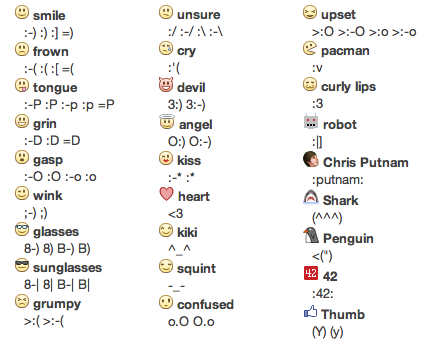
\includegraphics[width=0.5\textwidth]{ListofFacebookChatEmoji}
\caption{Некоторые графические смайлы, используемые в Facebook.}
\label{emoji}
\end{figure}

\pagebreak
Кроме ASCII смайлов есть ещё и графические --- это картинки, которые вставляются в текст. В
современных веб-сервисах и мобильных приложениях используется графический язык Emoji\footnote{www.emoji-cheat-sheet.com} для
записи слов, эмоций и действий. На рисунке \ref{emoji} изображены некоторые известные графические
смайлы, которые используются в социальной сети Facebook\footnote{facebook.com}. Обычно для
каждого из них есть ASCII аналог, причём не один. Набирая сообщение на клавиатуре компьютера или
ноутбука, удобнее поставить двоеточие со скобкой, но смартфоны и планшеты предоставляют все удобства
для вставки улыбчивых картинок: наряду с русской и английской клавиатурой, например, на них можно
подключить и клавиатуру графического языка Emoji.

Так как смайлы являются своего рода разметкой сообщений самими пользователями, их необходимо
использовать при анализе эмоциональной окраски. В этой работе будет рассмотрено применение
символьных и графических улыбок для сбора корпуса твитов и для предобработки данных непосредственно
перед классификацией.

\subsubsection{Хештеги}

Ещё одна особенность общения в микроблогах --- хештеги. Пользователь помечает в своём сообщении
слово, ставя перед ним <<\#>>, тем самым показывая связь объекта, обозначаемого этим словом, и всего
твита. Платформы для микроблогов предлагают возможность искать по хештегам, выбирать из них
популярные и следить за потоками актуальной информации. Многие хештеги используются в течение
короткого периода времени, но затем именно по ним можно найти информацию, которая когда-то была
актуальной и понадобилась через несколько месяцев. Например, организаторы мероприятий стараются
придумывать уникальный хештег, размещать его на информационных стендах, чтобы участники следили за
твитами друг друга и распространяли информацию по всему Интернету. Можно сказать, что это
повествовательная функция хештегов, точнее, тех из них, которые указывают на объект,~--- они могут
помочь осуществлять поиск сообщений на определённую тему.

Другую функцию этих специальных слов-ассоциаций можно назвать описательной. Именно такие хештеги
можно использовать в определении эмоциональной окраски текстов. В работе
\cite{qadir2013bootstrapped} предложен способ классифицикации хештегов по их эмоциональной
окраске. Авторы предлагают читателям посмотреть на 20 самых популярных хештегов из каждой
группы. Для наглядности в таблице \ref{tab:hashtags} приведены первые пять для каждой эмоции.

\begin{table}[h]
  \begin{tabular}{|c|c|c|c|c|} \hline
    \textbf{Привязанность} & \textbf{Ярость} & \textbf{Страх} & \textbf{Наслаждение} & \textbf{Грусть}\\ \hline
    \#youthebest&\#godie&\#hatespiders&\#thankinggod&\#catlady\\
    \#yourthebest&\#donttalktome&\#freakedout&\#thankyoulord&\#buttrue\\
    \#hyc&\#fuckyourself&\#creepedout&\#thankful&\#singleprobs\\
    \#yourethebest&\#getoutofmylife&\#sinister&\#superexcited&\#singleproblems\\
    \#alwaysandforever&\#irritated&\#wimp&\#tripleblessed&\#lonelytweet\\
    \hline
  \end{tabular}
  \caption{Самые популярные хештеги для пяти чувств: привязанности, ярости, страха, наслаждения и
    грусти. }\label{tab:hashtags}
\end{table}

Использование хештегов непосредственно для оценки эмоциональной окраски можно считать примерно таким
же, как и у смайлов, но лишь тогда, когда слово однозначно относится либо к положительным,
либо к отрицательным. В противном случае они либо становятся обычными словами: без символа <<\#>>
они участвуют в классификации наравне с другими, либо уточняют вероятность сообщения попасть в тот
или иной класс при помощи подсчёта условных вероятностей, где условием и является хештег.

\subsubsection{Сокращения, пролонгирования и пунктуация}
Тексты в микроблогах содержат не только уточняющую информацию, но и отчасти мешающую. Её нужно научиться использовать, так как
специфика сообщений не позволяет хоть что-то выкидывать.

Ограничение в 140 символов заставляет людей сокращать слова, причём как при помощи общеизвестных
аббревиатур, например, <<СПбГУ>> --- это Санкт-Петербургский Государственный Университет, так и при
помощи жаргонных конструкций: <<h8>> --- это на самом деле hate. На примере последнего видно, что
избавиться от этого слова было бы расточительно, но вряд ли <<h8>> внесло бы вклад в
вероятность сообщения попасть в класс отрцательных такой же, как и слово <<hate>>. Получается,
сокращения нужно уметь переводить.

Когда пользователям кажется, что длина сообщения не такая уж и маленькая, они используют
пролонгирования гласных --- ещё один способ выражать обеспокоенность темой твита. Автор преумножает
гласную в слове, изображая её продолжительное звучание, то есть, например, крик. Так <<nooooooo>>
будет, скорее всего, означать категорическое несогласие, а <<so cuuuute>> --- умиление. Таким
образом, каждое такое слово что-то значит, но классификатор может об этом не знать, значит, нужно
рассказывать классификатору какими-то другими способами, что это важное слово и какое из известных
является его менее эмоциональным аналогом.

Авторская пунктуация может рассказать об эмоциональной окраске сообщения не меньше, чем
смайлы. Например, в нейтральных твитах крайне редко встречаются восклицательные знаки. Впрочем,
однозначно классифицирующих особенностей пунктуации не так и много: наличие восклицательных знаков
указывает на наличие эмоциональной окраски, при этом нельзя без дополнительного анализа сказать,
какой именно; сочетание <<?!>>, скорее всего, будет означать недоумение, то есть классифицируется
как отрицательное; многоточия обычно говорят о нейтральности.

\subsection{Использование особенностей текстов для предобработки}\label{spec}
Смайлы, хештеги, сокращения, пролонгирования и пунктуация --- это то, про что классификатор уже не
знает, то есть перед подачей ему сообщения необходимо преобразовать это сообщение так, чтобы все
перечисленные особенности не выбивались и превратились в обычные слова.

Смайлы, перечисленные в таблице \ref{tab:smileys}, заменяются в тексте на соответствующую им
метку. Это делается для того, чтобы в обучающей выборке слово <<+>> встретилось больше раз среди
положительных твитов, тем самым, в вероятность попасть в класс положительных <<+>> даст больший
вклад, чем  просто <<:)>>. Так же, заменой на <<+>> и <<$\minus$>>, обрабатывается пунктуация.

К смайлам, заменяемым на метки, добавляется замена некоторых однозначно классифицирующихся
хештегов. Происходит это по той же причине, что и со смайлами. Если замена хештега не произошла, то
считается, что он должен стать обычным словом, то есть <<\#>> из начала пропадает, и дальше работа
происходит уже без учёта того, что это хештег.

Если в сообщении встречается неизвестное слово, его стоит проверить на наличие в словаре сокращений. В данной
работе используется словарь <<No slang>>\footnote{http://www.noslang.com/}, к которому программа
обращается во время подготовки данных к подаче классификатору. Запрос к словарю происходит в
онлайн-режиме, и для обработки сокращений нужно подключение к Интернету.

Повторения гласных убирать совсем не нужно: достаточно сократить количество повторяющихся гласных
до двух, то есть <<nooooooo>> заменится на <<noo>>. В этом случае слово <<noo>> может встретиться в
обучающей выборке, в отличие от <<nooooooo>>, где именно семь, а не восемь или девять букв
<<о>>. Таким образом слово <<no>> уже не то же самое, что <<noo>>, но все, сколько угодно длинные
продолжения гласной <<о>> сведутся к одному и тому же эмоциональному <<noo>>, которое даст каждому
из таких слов с продолжениями одинаковый повод попасть в класс <<$\minus$>>.



\section{Модель классификатора}
\subsection{Наивный байесовский классификатор}
\subsubsection{Описание классификатора}
Сперва рассмотрим простой случай преобразования твита в числовой вектор. Для этого построим словарь
на основе обучающих данных: каждое слово --- это отдельный признак,
который измеряется в конкретном сообщении. Пусть в тренировочной выборке было $D$ уникальных слов,
тогда числовой вектор, соответствующий твиту, выглядит следующим образом:
$\mathbf{x} = \{x_1,\ldots,x_D \}$. Здесь каждая компонента $x_j$ показывает, как представлено
$j$-ое слово в сообщении $\mathbf{x}$. Будем считать, что данные распределены по закону Бернулли, тогда
представленность слова определяется просто его наличием или отсутствием, то есть $x_j = 1$, если
$j$-ое слово встретилось в сообщении, и $0$ в противном случае. Задача --- сопоставить каждому такому
вектору наиболее правдоподобную метку класса, которую будем обозначать $y$. Множество всех классов
обозначим $\mathcal{C}$. Получается, что для каждого класса $c \in \mathcal{C}$ необходимо посчитать
функцию правдоподобия $p(\mathbf{x}|y=c)$. Наивный байесовский классификатор действительно наивен в
том смысле, что он предполагает независимость признаков. Это позволяет считать искомую вероятность
как произведение вероятностей для каждого признака:

\begin{equation}
  p(\mathbf{x}|y=c,\mathbf{\theta}) = \prod_{j=1}^Dp(x_j|y=c,\mathbf{\theta}_{jc})
  \label{eq:nbprob}
\end{equation}

Здесь $\mathbf{\theta}$~--- это матрица-параметр распределения Бернулли, который ищется на этапе
обучения классификатора, то есть по известным парам $\mathbf{x}, y$. На самом деле элемент этой
матрицы  $\mathbf{\theta}_{jc}$~--- это вероятность того, что $j$-ое слово встретится в примерах из класса $c$.


\subsubsection{Обучение и предсказание}
На этапе обучения классификтора нужно найти, как уже было сказано, параметры распределения,
моделирующего данные, и априорные вероятности классов $\mathbf{\pi}$. Сперва обозначим тренировочные
данные $\mathcal{D}$, тогда $\mathbf{x}_i \in \mathcal{D}$~--- это пример из обучающей выборки, а
$x_{i1},\ldots,x_{iD}$~--- количественные характеристики признаков для примера $\mathbf{x}$, и $y_i$~--- метка класса для него.

Посмотрим на $i$-ый пример, тогда вычисление вероятности пары $\mathbf{x}_i, y_i$ при условии
параметров $\mathbf{\theta}$ происходит по формуле:

\begin{equation}
  p(\mathbf{x}_i, y_i|\mathbf{\theta})
  = p(y_i|\mathbf{\pi})\prod_{j=1}^Dp(x_{ij}|\mathbf{\theta}_j)
  = \prod_{c\in\mathcal{C}}\pi_c^{\mathbb{I}(y_i=c)}
    \prod_{j=1}^D\prod_{c\in\mathcal{C}}p(x_{ij}|\mathbf{\theta}_{jc})^{\mathbb{I}(y_i=c)}
  \label{eq:mle}
\end{equation}

Переходя ко всему набору данных получается, что нужно максимизировать следующую величину

\begin{equation}
  p(\mathcal{D}|\mathbf{\theta})
  = \prod_{c\in\mathcal{C}}\pi_c
    \prod_{j=1}^D\prod_{c\in\mathcal{C}}\prod_{i:y_i=c}p(x_{ij}|\mathbf{\theta}_{jc})
  \label{eq:mleD}
\end{equation}

Теперь необходимо найти сответствующие этому максимуму параметры $\hat{\mathbf{\pi}}$
и $\hat{\mathbf{\theta}}_{ij}$. Произведя
все необходимые вычисления, получим, что
\begin{equation}
  \hat{\pi}_c = \frac{N_c}{N}
  \label{eq:pinb}
\end{equation}
\begin{equation}
  \hat{\theta}_{jc}= \frac{N_{jc}}{N_c}
  \label{eq:thetanb}
\end{equation}
В этих формулах $N$~--- количество примеров в обучающей выборке, $N_c$~---количество элементов в
классе $c$,
$N_{jc}$~--- количество раз, которое $j$-ое слово встретилось в примерах из класса $c$. Обучение
модели происходит за $O(ND)$ шагов.

Для предсказания класса $y$ для нового примера $\mathbf{x}$ необходимо максимизовать следующее
выражение по всем классам $c \in \mathcal{C}$

\begin{equation}
  \hat{\pi}_c\prod_{j=1}^D(\hat{\theta}_{jc})^{\mathbb{I}(x_j=1)}(1-\hat{\theta}_{jc})^{\mathbb{I}(x_j=0)}
  \label{eq:predict}
\end{equation}

Класс, для которого оно получилось максимальным, и считается наиболее правдоподобным для данного
примера.

\subsubsection{Проблемы подхода}

Основная проблема описанного подхода заключается в том, что не обязательно все слова (признаки)
встретятся во всех классах. Например, если $j$-ое слово не представлено в классе $c$, то $N_{jc}=0$
и вероятность того, что рассматриваемое сообщение попадёт в класс $c$ тоже станет нулевой. От этой
проблемы может избавить переход к байесовскому подходу, когда параметры становятся случайными
величинами со своими распределениями. Ещё для устранения этой проблемы
используется сглаживание Лапласа\cite{field1988laplacian}, когда и к
числителю, и к знаменателю прибавляется по $1$.
Это частный случай байесовского подхода.

Другая проблема, с которой необходимо бороться,~--- это невозможность расширения словаря: если слова
не было в обучающей выборке, то классификатор снова сталкивается с нулевыми вероятностями, но теперь
для всех классов.

\subsection{Вероятностная модель нового метода}
\subsubsection{Переход к байесовскому подходу}\label{bnb}
Чтобы избавиться от проблемы с нулевыми вероятностями <<честным>> способом, перейдём к байесовскому
наивному байесовскому классификатору. В этом случае параметры вместо точечных величин представляются
случайными величинами с априорными распределениями. В модели классификатора параметры --- это
вероятности, то есть их значения ограничены на отрезке $[0,1]$. Так распределение для каждого из
параметров должно задавать случайную величину, ограниченную на отрезке. Для моделирования параметра
$\mathbf{\pi}$ будем использовать распределение Дирихле $\operatorname{Dir}(\mathbf{\alpha_0})$, которое
устанавливает закон распределения многомерной случайной величины, где все компоненты~--- величины из
отрезка $[0,1]$ и суммируются в $1$. Считаем также, что каждый из параметров $\theta_{jc}$ имеет
Бета-распределение на отрезке $[0,1]$ $\operatorname{Beta}(\beta_0,\beta_1)$. Все параметры
считаются независимыми, поэтому априорная вероятность параметров считается по формуле
\begin{equation}
  p(\mathbf{\theta}) = p(\mathbf{\pi})\prod_{j=1}^D\prod_{c\in\mathcal{C}}p(\theta_{jc})
  \label{eq:apr}
\end{equation}
Задача теперь получить апостериорную вероятность на основании данных $\mathcal{D}$ из обучающей
выборки и выяснить, попадёт ли она в тот же класс, что и априорная, то есть получится ли для неё
выражение вида
$\operatorname{Dir}(\ldots)\cdot\operatorname{Beta}(\ldots)\cdot\ldots\cdot\operatorname{Beta}(\ldots)$.
По теореме Байеса искомую вероятность можно посчитать по следующей формуле
\begin{equation}
  p(\mathbf{\theta}|\mathcal{D}) =
  \frac{p(\mathbf{\theta})\cdot p(\mathcal{D}|\mathbf{\theta})}{p(\mathcal{D})}
  \label{eq:apo}
\end{equation}
Знаменатель выражения не зависит от параметров, поэтому рассмотрим отдельно числитель. Если
расписать плотности распределений и сгруппировать полученные произведения, получится вывод,
сокращённая версия которого приведена ниже. $M$ здесь некоторая постоянная.
\begin{align}
  p(\mathbf{\theta}) \cdot p(\mathcal{D}|\mathbf{\theta})
  & =  M\cdot\prod_{c\in\mathcal{C}}\pi_c^{\alpha_0c-1}\cdot
  \prod_{j=1}^D\prod_{c\in\mathcal{C}}\theta_{jc}^{\beta_0}(1-\theta_{jc})^{\beta_1}\cdot
  \prod_{\mathbf{x}\in\mathcal{D}}\prod_{c\in\mathcal{C}}\pi_c\prod_{j=1}^D\theta_{jc}^{x_{jc}} \label{eq:plo1}\\
  & = M\cdot\prod_{c\in\mathcal{C}}\pi_c^{\alpha_{0c}+N_c}\cdot
  \prod_{c\in\mathcal{C}}\prod_{j=1}^D\theta_{jc}^{\beta_0+N_c-N_{jc}}(1-\theta_{jc})^{\beta_1+N_{jc}}
  \label{eq:plo2}
\end{align}
В выражении \label{eq:plo2} записано не что иное, как произведение плотностей распределения Дирихле и
Бета-распределений. Так вероятность $p(\mathbf{\theta}|\mathcal{D})$ осталась в том же классе, что и
$p(\mathbf{\theta})$.

\begin{align}
  p(\mathbf{\pi}|\mathcal{D}) &= \operatorname{Dir}(N_1+\alpha_{01},\ldots,N_c+\alpha_{0c},\ldots)\label{eq:pi}\\
  p(\theta_{jc}|\mathcal{D}) &= \operatorname{Beta}(N_c-N_{jc} + \beta_0, N_{jc}+\beta_1) \label{eq:thetajc}
\end{align}
Обозначим получившиеся параметры как $\alpha_0^*$, $\beta_0^*$ и $\beta_1*$ соответственно.

Остаётся понять, как при помощи полученных данных можно предсказать класс для новых
примеров. Рассмотрим пример $\mathbf{x}$. Хотим найти для него значение метки $y$. Для этого нужно
максимизировать $p(y=c|\mathbf{x},\mathcal{D})$ по всем $c\in\mathcal{C}$.

\begin{equation}
  p(y=c|\mathbf{x},\mathcal{D}) =
  \frac{p(y=c|\mathcal{D})\cdot p(\mathbf{x}|y=c,\mathcal{D})}{p(\mathbf{x}|\mathcal{D})}
  \label{eq:bnbpred}
\end{equation}

Снова будем смотреть только на числитель. Первый его множитель на самом деле является математическим
ожиданием $\pi_c$ по $\mathbf{\pi}$ c плотностью распределения Дирихле. Краткая версия вывода
приведена ниже, в \ref{eq:mathpi1}, \ref{eq:mathpi2} и \ref{eq:mathpi3}. Здесь для
преобразования \label{eq:mathpi1} используется техника маргинализации, а переход к \ref{eq:mathpi3}
следует из определения математического ожидания.
\begin{align}
  p(y=c|\mathcal{D})&=\int_{\mathbf{\pi}\in\Pi}p(y=c,\mathbf{\pi}|\mathcal{D})d\mathbf{\pi}\label{eq:mathpi1}\\
  &= \int_{\mathbf{\pi}\in\Pi}p(\mathbf{\pi}|\mathcal{D})p(y=c|\mathcal{D},\mathbf{\pi})d\mathbf{\pi}\label{eq:mathpi2}\\
  &= \underset{\mathbf{\pi}\sim\operatorname{Dir(\alpha_0^*)}}{\mathbb{E}}\pi_c
  \label{eq:mathpi3}
\end{align}

Аналогично первому разбираем второй множитель. Снова воспользуемся техникой маргинализации
для записи \ref{eq:maththeta1}. Теперь раскрываем вероятность  в произведение вероятностей
--- так можно делать, потому что величины $x_i$ и $\theta_{*c}$ независимы, и получаем
 формулу~\ref{eq:maththeta2}. Далее переписываем интеграл в обозначениях математического ожидания и, согласно
посчитанному ранее, приходим к тому, что благодаря независимости параметров получили произведение
математических ожиданий случайных величин $\theta_{jc}$ с плотностью Бета-распределения.

\begin{align}
  p(\mathbf{x}|y=c,\mathcal{D}) &=\int_{\theta\in\Theta}p(\mathbf{x},\theta_{*c}|y=c,\mathcal{D})d\theta_{*c}\label{eq:maththeta1}\\
  &=\int_{\theta\in\Theta}p(\mathbf{x}|y=c,\mathcal{D},\theta_{*c})p(\theta_{*c}|y=c,\mathcal{D})d\theta_{*c}\label{eq:maththeta2}\\
  &=\underset{p(\theta_{*c}|y=c,\mathcal{D})} {\mathbb{E}}p(\mathbf{x}|y=c,\mathcal{D},\theta_{*c})\label{eq:maththeta2}\\
  &=\prod_{j=1}^D\underset{\theta_{*c}\sim\operatorname{Beta}(\beta_0^*,\beta_1^*)}{\mathbb{E}}\theta_{jc}^{x_{ij}}
\end{align}

Так как параметры вычислены на этапе обучения, а формула математических ожиданий для
соответствующих распределений известна, остаётся только подставить их в выражение \ref{eq:bnbpred},
максимум которого мы ищем.

\subsubsection{Использование n-грамм для измерения признаков}\label{ngram}
Альтернативный взгляд на подсчёт вероятностей сообщений --- это разбиение сообщения на $n$-граммы, то
есть $n$-буквенные сочетания. Такое изменение позволит искусственно ослабить требование о
независимости признаков. Допустим, что исходное сообщение разбивается на триграммы. Три здесь выбрано,
так как вычислительно количество всех возможных триграмм ещё не так велико, но уже информативно.\footnote{
А также по причине того, что длина слов в английском языке  в
среднем около пяти букв \cite{balota2007english}. Это значит, что, чтобы не учитывать
слово целиком, можно разбить его на две части, первая из которых
будет служить ещё и контекстом для предыдущего слова.
}
Переобозначим $x_i$, теперь они представляют триграммы. Пусть триграмм в сообщении всего $L$, тогда
вектор $\mathbf{x} = {x_1, \ldots, x_L}$ описывает представленность триграмм в сообщении.
Вероятность того, что сообщение попадёт в класс $c$, в этом случае подсчитывается по следующей формуле

\begin{equation}
  p(\mathbf{x}, y=c) = \prod_{j=2}^Lp(x_j|x_{j-1},y=c)
\end{equation}

Модель классификатора немного изменится, а новыми параметрами станут как раз\\
$p(x_j|x_{j-1},y=c)$, которые и будет искать алгоритм на этапе обучения.

Перейдём к предыдущим обозначениям и выясним, как изменятся формулы подсчёта параметров и
искомой. Вектор $\mathbf{x}$ снова показывает представленность каждой триграммы из обучающей
выборки в рассматриваемом примере: $1$ стоит на месте присутствующей триграммы и $0$ на месте
отсутствующей. Введём также функцию, которая поможет понимать последовательность триграмм в примере:
$n(x_{j})$ показывает, какой по счёту встретилась $j$-ая триграмма в примере. Если не встретилась,
то пускай значение этой функции будет $-\infty$. Для простоты считаем,
что каждая триграмма встретилась только один раз. В формуле пересчёта параметра $\mathbf{\pi}$ \ref{eq:pi} ничего не изменится, так как
на априорные вероятности класса изменение не повлияет. Пусть $D$~--- это теперь количество всех
триграмм, встретившихся в обучающей выборке. Дополнительно обозначим $N_{jkc}$~---
количество пар из триграммы с номером $k$ и следующей прямо за ней триграммы с номером $j$ в классе $c$.
$\theta_{jkc}$~---~вероятность встретить триграмму с номером $k$ сразу за триграммой с номером $j$ в
классе $c$. Тогда пересчёт параметра $\theta_{jkc}$ будет производиться по формуле, аналогичной
\ref{eq:thetajc}, но с учётом связи триграмм.

\begin{equation}
  p(\theta_{jkc}|\mathcal{D}) = \operatorname{Beta}(N_c-N_{jkc}+\beta_0, N_{jkc}+\beta_1)
  \label{eq:thetajkc}
\end{equation}

Новые параметры опять обозначим $\beta_0^*$ и $\beta_1^*$ для удобства. В формуле \ref{eq:bnbpred} снова будем смотреть только на числитель. Первый множитель не изменится,
а второй будет вычисляться так

\begin{equation}
   p(\mathbf{x}|y=c,\mathcal{D}) =
   \prod_{j=1}^D\prod_{k=1}^D\underset{\theta_{**c}\sim\operatorname{Beta}(\beta_0^*,\beta_1^*)}{\mathbb{E}}\theta_{jkc}^{\mathbb{I}(n(x_{j})=n(x_{k})+1)}
   \label{eq:maththetagr}
\end{equation}

Причём получится, что каждое $\theta_{jkc}$ представлено не больше, чем один раз, так как в примере
за триграммой может следовать только одна другая.


\section{Реализация}
\subsection{Онтологии для замены неизвестных слов}\label{ontology}
Способ содержательного устранения проблемы с неизвестностью слов в анализируемых примерах,
предлагаемый в работе, --- это использование онтологий. Онтологией называется некоторая схема области
знаний, обычно она представляет собой направленный ациклический граф, вершины которого ---
понятия. Чем выше в графе находится вершина, тем шире соответствующее ей понятие. Таким образом,
если в сообщении встретилось слово, которое классификатору неизвестно, его можно заменить на более
общее понятие в соответствии с онтологией.

База знаний Википедии\footnote{https://www.wikipedia.org/} составляется пользователями и на данный
момент содержит 4515000 статей только на английском языке. Структура организации статей в
Википедии похожа на то, что мы ищем, --- это граф категорий.
На основе категорий Википедии уже составлена онтология проектом DBpedia\cite{dbpedia-swj} --- она и
используется в работе.

Данные выкачиваются в формате
Turtle\footnote{http://www.w3.org/TR/turtle/}. У нас есть два файла: первый --- отображение статей в
подмножество категорий, второй --- лес всех категорий. Граф категорий сильно несвязный, большинство
из них не участвуют ни в какой иерархии. Согласно этим особенностям нужно решить задачу хранения
онтологии и поиска нужной категории.

В первую очередь, стоит сказать, что хранится отображение категорий в номера вершин в графе, так как
хранить целые строчки для такого количества данных неэкономно. Эти отображения кладутся в
бор\footnote{Marisa trie: https://code.google.com/p/marisa-trie/}, в
соседнем боре запоминаются отображения статей в категории. Пример можно увидеть на рисунке \ref{ontology}.
Когда появляется неизвестное слово, ищется статья, где искомое
слово --- префикс, так как названия статей не всегда из одного слова.
Выбираем из всех категорий, к которым относится данная статья, ту, что в иерархии находится ниже всего. При равенстве уровня выбираем любую.

\begin{figure}
  \centering
  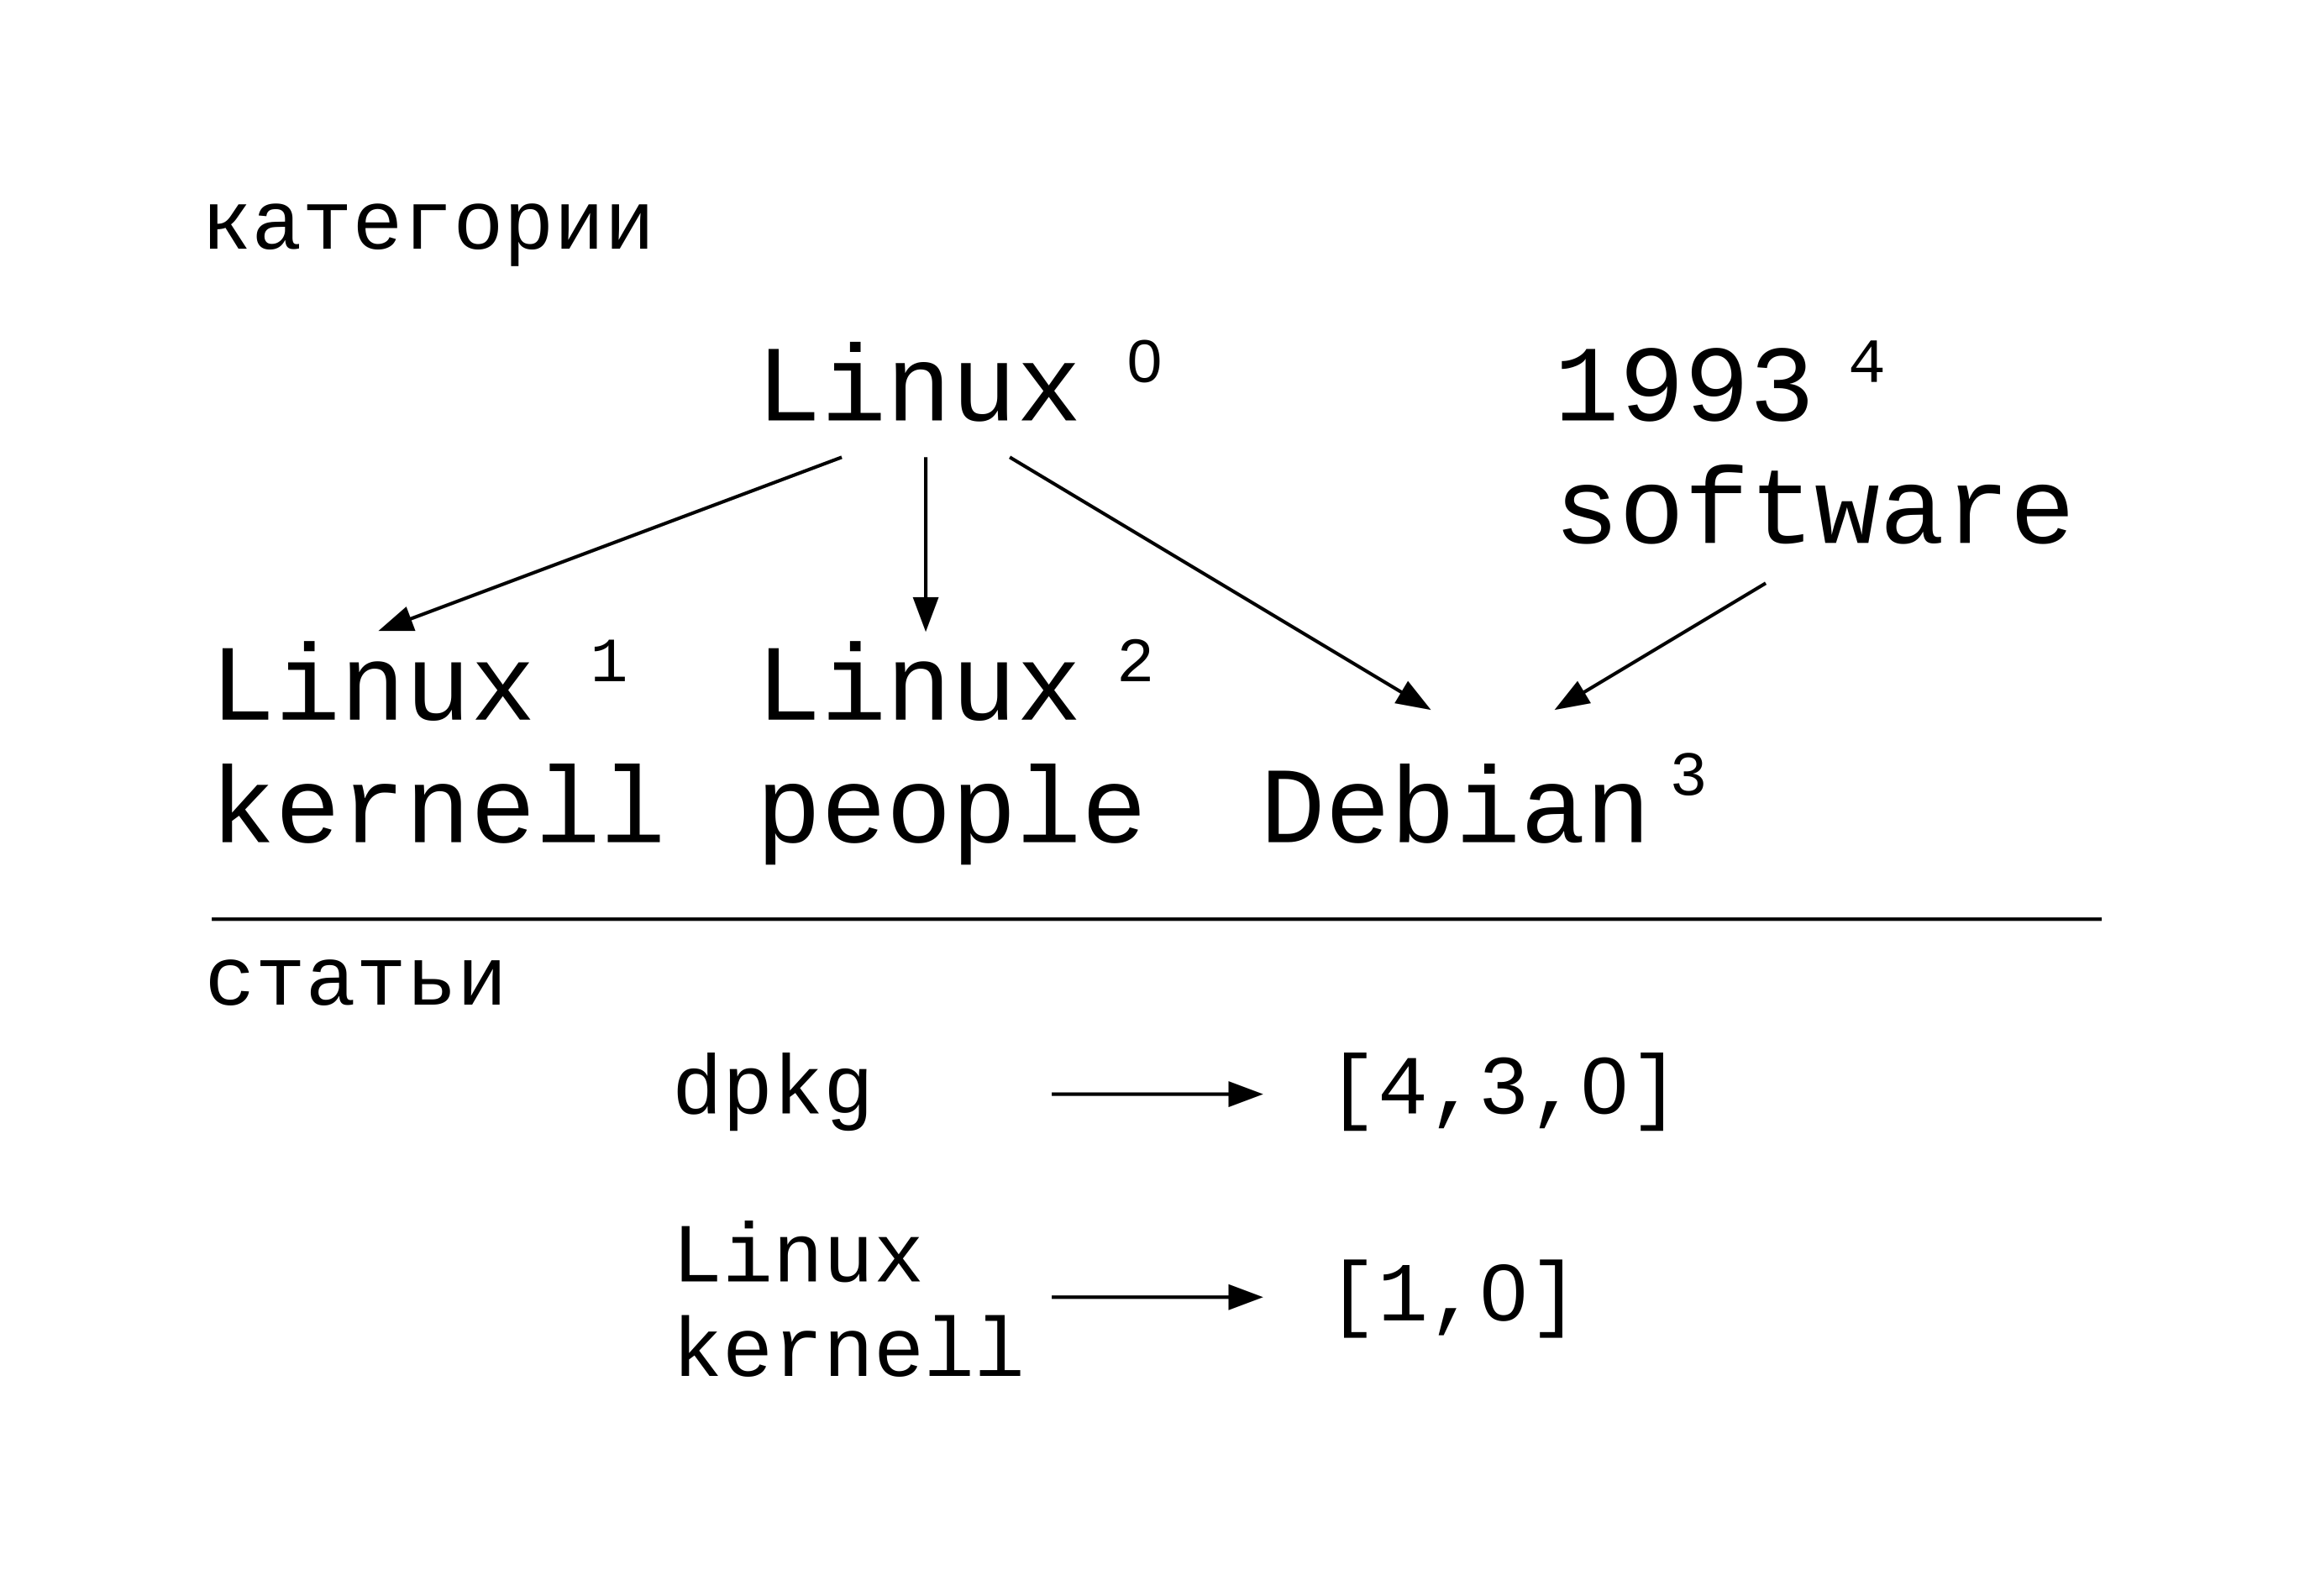
\includegraphics[width=0.5\textwidth]{ontology}
  \caption{Хранение статей <<Linux kernell>> и <<dpkg>> с некоторыми связанными с ними категориями.
Сверху -- бор категорий, снизу -- отображения статей. <<Linux kernell>> здесь
присутствует два раза, так как есть такая категория и одноимённая ей статья.}\label{ontology}
\end{figure}

\subsection{Алгоритмы подготовки данных, предсказывания и обучения}
Описанные в ходе данной работы идеи были объединены в метод классификации
и реализованы на языке Python с использованием его расширения Cython. Ниже
приведена последовательность действий со ссылками на разделы в тексте, где про эти действия
рассказывается более подробно. Некоторые моменты не были разъяснены ранее, поэтому им уделяется чуть
больше внимания. Отдельно рассмотрим три части: подготовка данных, обучение классификатора,
предсказание класса.

\textbf{Подготовка данных} (некоторые пункты не относятся к данным из обучающей выборки, в этом
случае в конце пункта стоит <<*>>):
\begin{itemize}
  \setlength{\itemsep}{1pt}%
    \setlength{\parskip}{1pt}
  \item замена сущностей html на слово <<URL>>, упоминаний пользователя на <<USER>> и чисел на <<42>>;
  \item перевод сообщения в нижний регистр;
  \item замена смайлов, хештегов и некоторых знаков препинания на <<+>> или <<$\minus$>> (раздел \ref{spec});
  \item замена долгого повторения гласных на сочетание из двух букв (раздел \ref{spec});
  \item разбивка на слова с учётом знаков препинания при помощи Penn Treebank Tokenizer из NLTK\cite{bird2006nltk};
  \item замена сокращений на их расшифровки (раздел \ref{spec});
  \item замена неизвестных классификатору слов на обобщения каждого из них (раздел \ref{ontology});*
  \item приведение всех слов к начальной форме при помощи алгоритма Snowball
  Stemmer\cite{porter2001snowball}
  \item удаление артиклей, предлогов и союзов из сообщения.
\end{itemize}

\textbf{Обучение классификатора:}
\begin{itemize}
  \setlength{\itemsep}{1pt}%
    \setlength{\parskip}{1pt}
\item подготовка данных и сохранение множества известных слов;
\item преобразование полученных строк на перекрывающиеся пары триграмм\footnote{Из предложения
    \texttt{\textbf{Мама\_мыла\_раму.}} получатся следующие пары триграмм: \texttt{\textbf{Мам|а\_м}},
    \texttt{\textbf{а\_м|ыла}}, \texttt{\textbf{ыла|\_ра}}, \texttt{\textbf{\_ра|му.}}}, теперь одна пара триграмм --- это признак, по которому измеряются сообщения;
\item каждый пример из обучающей выборки преобразуется в числовой вектор: на месте соответствующей
  пары триграмм из набора ставится $1$, если она есть в примере, и $0$, если нет;
\item поиск апостериорных распределений параметров согласно формулам \ref{eq:pi} и \ref{eq:thetajkc}.
\end{itemize}

\begin{samepage}
  \textbf{Предсказание класса для нового примера:}
  \begin{itemize}
    \setlength{\itemsep}{1pt}%
    \setlength{\parskip}{1pt}
  \item подготовка примера согласно описанному выше в <<Подготовка данных>>;
  \item преобразование полученной строки на перекрывающиеся пары триграмм;
  \item преобразование полученного набора в числовой вектор: на месте соответствующей
    пары триграмм из набора ставится $1$, если она есть в примере, и $0$, если нет;
  \item вычисление вероятности примера оказаться в каждом из классов (<<$1$>> или <<$-1$>>) согласно выражению
    \ref{eq:bnbpred} и вычислению множителей из неё по \ref{eq:mathpi3} и \ref{eq:maththetagr}
  \item выбор класса, который дал наибольшую вероятность попадания в него.
  \end{itemize}
\end{samepage}


\section{Количественная оценка метода}\label{compare}

Твиттер предоставляет API\footnote{https://dev.twitter.com/} для извлечения и поиска сообщений, в
том числе по поисковому запросу. Ответом на запрос к Твиттеру является набор сущностей, каждая из
которых хранит информацию о сообщении: его id, текст, имя пользователя-автора,
время публикации, а также, если оно является ответом или ретвитом другого, то указывается id
``родительского'' твита. В таком виде не восстановить цепочки твитов: чтобы найти диалог
между пользователями, нужно обойти все существующие твиты и найти из них те, которые ссылаются на
определённое сообщение, -- так можно найти все ответы на него или его ретвиты. Скорее всего, если
найден некоторый твит про объект, то ответы на него будут про этот же объект, то есть вычислять
ответы необходимо.

Предлагается делать это следующим образом. Пусть есть твит $T$, его id $T_{id}$, имя пользователя,
который его опубликовал $T_{user}$, и время публикации $T_{time}$. Отличительная особенность ответов
в Твиттере, как говорилось ранее, -- это упоминания, то есть ответ на твит пользователя с именем username
будут начинаться со строки ``@username''. Тогда, чтобы найти все ответы на твит $T$ будем искать не
по множеству всех возможнных сообщений, а по всем сообщениям, опубликованным позднее $T_{time}$ по
поисковому запросу ``@$T_{user}$''. Среди них уже можно будет выделить сообщения, которые ссылаются
на твит с номером $T_{id}$ -- это и будут все ответы на $T$.

Так собираются данные по слову-запросу для разметки эмоциональной окраски актуальных сообщений по
этой теме. Этот метод использовался для расширения тестовой выборки, используемой для анализа
алгоритмов в ходе всей работы.

Для обучения классификатора использовались 1000000 размеченных сообщений. Классификаторы сравнивались
на 386 тестовых примерах, 204 из которых отрицательные, 182 -- положительные.

\begin{table}[h]
    \centering
    \begin{tabular}{|c|c|c|c|c|}
      \hline
      \textbf{Метка класса} & \textbf{Precision} & \textbf{Recall} & \textbf{F1-score} &
      \textbf{Количество} \\ \hline
      -1.0&0.82&0.75&0.78&204\\ \hline
      1.0&0.74&0.82&0.78&182\\ \hline \hline
      avg / total&0.79&0.78&0.78&386\\
      \hline
    \end{tabular}
    \caption{Классификация наивным байесовским классификатором}\label{tab:nb1}
\end{table}
\begin{table}[h!]
    \centering
    \begin{tabular}{|c|c|c|c|c|}
      \hline
      \textbf{Метка класса} & \textbf{Precision} & \textbf{Recall} & \textbf{F1-score} &
      \textbf{Количество} \\ \hline
      -1.0&0.88&0.74&0.80&204\\ \hline
      1.0&0.75&0.88&0.81&182\\ \hline \hline
      avg / total&0.82&0.81&0.81&386\\
      \hline
    \end{tabular}
    \caption{Классификация байесовским наивным байесовским классификатором с триграммами и онтологиями}\label{tab:bnb}
\end{table}

В таблицах \ref{tab:nb1} и \ref{tab:bnb} приведено сравнение базового классификатора и его
изменённой версии, основанной на байесовском подходе и использовании триграмм и онтологий. Новый
классификатор дал улучшение предсказания на $3\%$, при этом метод не перестал быть инкрементально
обучающимся, то есть его можно уточнять в онлайн-режиме.


\section*{Заключение}

Отдельно стоит выделить следующие результаты.
\begin{itemize}
\item Проведено сравнение базовых методов обучения с учителем: наивный байесовский классификатор,
  метод опорных векторов и логистическая регрессия --  для данных из микроблогов по
  параметрам точности, полноты результатов и времени обучения. Подробнее о сравнении написано в
  разделе \ref{comparemeth}. Лучше всех себя показал наивный байесовский классификатор, время
  обучения которого на порядок ниже двух других.
\item Проанализированы особенности задачи анализа мнений для микроблогов, найдены варианты
  использования этих особенностей для улучшения методов классфикации. Об использовании особенностей
  написано в разделе \ref{spec}.
\item На основе наивного байесовского классификатора предложен, обоснован и реализован новый
  метод. Для улучшения использовались: переход к байесовскому подходу (модель описана в разделе
  \ref{bnb}), триграммы для использования информации о связи слов в предложении (раздел \ref{ngram})
  и онотологии на базе категорий из Википедии (раздел \ref{ontology}).
\item Сравнение нового метода с базовым проведено на тех же данных, что и сравнение методов обучения
  с учителем. Разработанный метод дал улучшение на $3\%$ (раздел \ref{compare}).
\end{itemize}


% Библиография
\printbibliography

\end{document}
